\chapter{High Data Complexity Power/EM 1} \label{cha:High Data Complexity Power/EM 1}

So far, we've attacked two cryptographic systems in the course:
\begin{itemize}
    \item RSA using Montgomery reduction with time as a side-channel
    \item AES using simple power analysis
\end{itemize}

We attacked AES using simple power analysis, we had as an input a power trace
consist of hundreds of thousands of points and then we actually wrote a
classifier or let's say dozen of classifiers and the classifier takes as input
the power traces and outputs what is the hamming weight of the first byte of the
state, and what was the hamming weight of the second byte of the state and so
on\ldots

\begin{table}
    \caption{Hamming weights of different bit strings~\cite{hamming}}\label{hammingWeights}
    \begin{center}
    \begin{tabular}{ cc }
        \toprule
        String & Hamming Weight \\ 
        \midrule
        11101 & 4 \\ 
        11101000 & 4 \\
        00000000 & 0 \\
        789012340567 & 10 \\
        \bottomrule
    \end{tabular}
    \end{center}
\end{table}

For AES you have 84 of this classifiers and we didn't actually talked about how
these classifier are constructed but you can assume they take as input that
power trace and output the hamming weight. 

A question arise: does the classifier look at the entire power trace? let's say
I have a classifier that wants to find out the hamming weight of the first
sub-bytes operation of AES so you take the first byte of the plain text start
with the first byte of the key and then you do sub bytes on this byte: you go to
that sub bytes table and you replace the state with sub bytes of the state. 

Do you think that this classifier needs to look at the entire 1000 or 100,000
points of the trace? Or maybe it needs to look at the certain limited amount of
points in the trace? The answer is that our given power trace contains a lot of
redundant information. We start our measurement a while before the first
sub-byte operation happens, and therefore there are a lot of points in the data
which is irrelevant for us (just an arbitrary operations that happened before
the encryption started).

So lets assume we have an army of classifiers, each one of these classifiers is
going to be look at the certain points of the trace maybe 10 or 15 or hundred
points in this very very large power traces. How can we know to find at which
point to look at? We haven't taught that yet and we will go into that a little
bit during this lecture. 
 
Now, we want to combine the two attack methods: timing and simple power analysis
and take the best part of each one of these methods combining them somehow and
the results is going to be called differential power analysis.
 
When we did a timing attack what was our threat model? What was the adversary
allowed to do? We was allowed to send inputs to the device and get the outputs
from the device and measure how long it took.
 
We weren't necessary in control of the inputs we just had to know when the input
was provided we didn't have to know what the input was. We just needed to know
when was the input when was the output and find the time difference. We had to
measure a lot of times and have many inputs, and then we did some statistics to
analyze it. The various scenarios when we can justify a timing attack – when the
device is in your position, or it's accessible across the web and so on.

What about simple power analysis? What was the threat model there? What we
allowed to do with the device? First of all we had to open the device and cut it
power supply and connect a power probe which is the meter that measures the
power consumption, this is an invasive attack so maybe it's considered less
probable that we actually allowed to do that as attackers. If you are doing an
electromagnetic probe it would be less invasive but you still will have to get
very close to the device, but it would be less detectable. 

But what else we had to do before we perform simple power analysis? And now I'm
reminding you what I just said couple of minutes ago, how do we actually do a
simple power analysis, we have an army of classifiers, where this classifier
came from? We need to train them. who do we train classifiers? we give them a
lot of labeled data, we need to do what is called: \textit{profiling}, which
means we have to get really good understanding of the DUT. How do we get this
understanding? We have an offline phase. We have a device to which we can do
reverse engineering and get really into it's internals. Maybe look at it with a
microscope or we can understand completely how it works and then this device
this similar to the DUT. The only things we're not allowed to know as adversary
is the secret key.

What is the difference between two devices? according to the Kirchhoff's
principles the difference between our DUT to what we use to learn is the
\textit{current}. 
  
Now, one might ask: how do we get this copy of the device in the real world?
well, we can buy it, we can steal it, maybe buy it online. you have to have a
very involve offline phase before you can do a simple power analysis you have to
get close to the device and do a reverse engineering if an justify it by buying
stuff on eBay you can go to the trash you can look at the data sheets and so on.

Next thing in our attack is the \textit{online phase}. In simple power analysis
you can perform one or two simple measurements and what is the problem with
these measurements  is that it's our only chance to measure and we have one
trace that have to be very clean with very little noise. And of course, we can't
really control this noise. For example if we're doing this outside the lab
there's going to be some kind of noise, but if we are using measurement
equipment the measurement equipment is going to introduce noise to and the DUT
is introducing noise by it self. Unfortunately, we can't do so much about the
noise in the simple power analysis scenario because we only have the online
phase.

\subsubsection{What can we do if we had a little noise and we don't have the exact key?}

\textit{That's exactly our problem with simple power analysis}

Maybe only one byte is incorrect and we might try to search for the key around
the guess? Let's do a little bit of combinatorics: let's say I got AES key which
is 16 bytes long and it's 8 bit implementation and I tried the key and it's
wrong. Now, I'm trying to see if I change one byte in the key maybe that will
fix the key. So, how many attempts well I have to perform? Lets try to change
the byte with index 0 to all possible values, then change at index 1, then 2 and
so it goes\ldots How many decryptions should we do? We have 256 per position
times the 16 bytes of the key. And if that didn't work I didn't find a key,
maybe I'll try 2 bytes combinations, so how many attempts I'll have to do now?
It's 16 choose 2 which is more or less 16 squared so it's two to the power of
$4\times2$. So I chose to byte and then what I do is that I go over all the
possible combination of this bytes which is two to the power of 16 so it is two
to the power of $8+8=16$. It grows up really fast and it's going to be as bad as
brute force pretty quickly. And what if I have to change tree bytes? it's going
up so I have to work very very hard if I don't get the key right it blows up
exponentially. One might ask why we are talking about bytes and not bits? if we
are looking at a 8 bit micro-controller a lot of the operations are going to be
byte oriented so it's going to be more likely to get the entire byte wrong. So
if I don't have the key right I am in trouble and I have to search and search
very very hard. 

\textbf{The solution to this problem is to have a more complex offline phase which prepare us to the online phase.}

Simple power-analysis will work just fine if it's reasonable to conduct
thousands of measurement on the same device in order to eliminate noise with
statistics, however, it's not always practical.

\section{High Data Complexity Attacks}

(AKA: \textit{DPA} and \textit{CPA})

The main idea is to capture many traces and use statistics to recover the key.
The advantages of this methods are:
\begin{itemize}
    \item Doesn't require detailed information about DUT (save us the cost of
    doing reverse engineering to the device)
    \item Succeeds even under extreme noise
\end{itemize}

On the other hand, the drawback is that the attack model is different now, we
need to own the device. That may cause some people to think that this attack
model is irrelevant because it's not practical. In truth, it might be practical
in a quite wide range of situations.

\subsubsection{Why would we want to get the secret of somebody else?}

A good example for it is how TV suppliers calculate your bill. You've a secret
and you use it to identify yourself to the supplier. Based on that, the supplier
should decide which TV shows you have access to, and how to charge you in case
you watch paid TV shows, use VOD and etc\ldots If someone get his hand on your
password, he can use it to watch whatever TV shows he wants at whatever cost,
because you're the one to pay the bill.

\subsection{How complex power analysis actually works}

Until now, we knew about 2 ways of attacking with side channel:
\begin{enumerate}
    \item \textit{Timing Attack}
    \item \textit{Simple power analysis}
\end{enumerate}

When we used timing attack, we tried many input, and the measurement for each
input contained 1 output: for 1 input we had the time it took. On the other
hand, when we did Simple Power Analysis, for each input we had a huge power
trace (vector of points which indicates the power consumption over time for a
given input). In other words, the data complexity was simple in both of these
methods - we had a $1d$ input. Now we'll try to take it a step further and
combine these methods and create a new method with $2d$ input, which mean now we
have high data complexity. Instead of giving just the power trace, we'll give as
an input the traces for various data at a fixated points in time. We have a set
of data ${D_1, D_2, ..., D_n}$ and we have the power trace of the system for
each one of these inputs, at the the time, i.e. the first point in the power
trace for all these inputs, was taken at the same relative time. So now our
output isn't a vector but rather a Matrix $M_{DxT}$.

\begin{figure}[!ht]
    \centering
    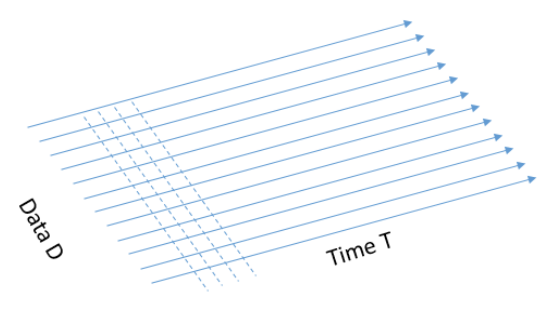
\includegraphics[width=0.8\textwidth]{images/Lecture6/DPA_Illustration.png}
    \caption{many measurements over time} \label{fig:DPA_Illustration}
\end{figure}

The suspicious reader should ask: how it's possible that we measure the
power-traces of all the different data inputs all at the same time? That is
indeed a challenge to align all the measurement along the time-line and some of
the countermeasures to the attack we present here, will insert randomized
operations or will change the clock speed so that we'll have trouble to align
the power-traces along the time-line. If you're curious about that, you might
find it interesting to look on the DPA book (the course book) and read about the
countermeasures and the ways to overcome them.

\subsection{Using the Vaizata method}
The next thing we're going to do is to use the Vaizata similarly to how we did
it with timing attacks. When we did timing attack, we made a guess about a bit
of the key and then we measured how much time it took. Now, we're going to make
an assumption that at sometime, the algorithm depends on the key, therefore the
power consumption will be depended on the key. Finally we're going to check it
with the measurements using some statistics. 

Unlike the timing attack where we knew that we measure the relevant data, when
we used power analysis, we have a very long power trace where only few points
relevant to us and all the other points represent data which isn't related to
the key.

\begin{figure}[!ht]
    \centering
    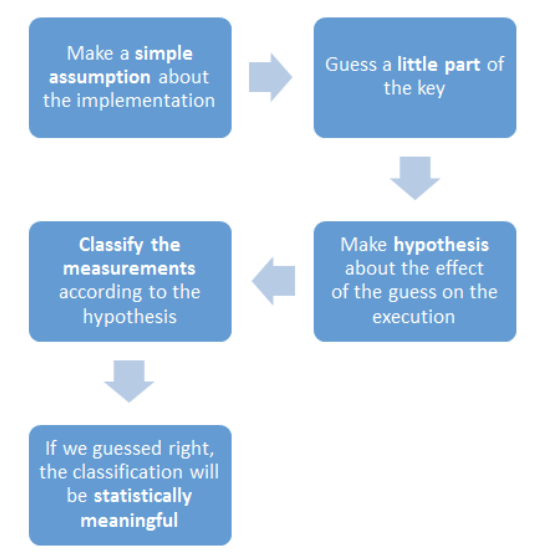
\includegraphics[height=0.9\textwidth]{images/Lecture6/vaizata.png}
    \caption{Vaizata method stages} \label{fig:vaizata}
\end{figure}

Now, we're looking for a stage during the AES algorithm, where a small amount of
bits of the key, affect large amount of the bits in the state. The intuition
here is that we want to find a stage in the algorithm, where the power
consumption depends on the key value.

\begin{figure}[!ht]
    \centering
    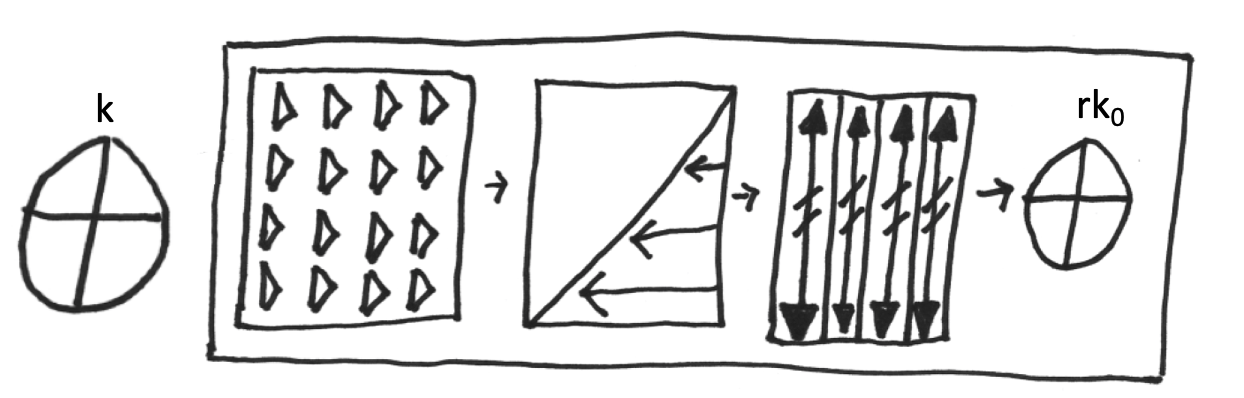
\includegraphics[width=0.8\textwidth]{images/Lecture6/AES-stages-figure.png}
    \caption{AES stages} \label{fig:aes-stages}
\end{figure}

We might consider measuring the power consumption just before the start of the
algorithm, but in this case the key has no affect on the state. Next, we have
the add round key. After this operation, each bit of the key affect exactly one
bit of the state. Why is that? because we essentially ``XOR" the key with the
state, which so the the bit $k[0]$ affects the bit $s[0]$.

Our second operation will be the \texttt{subbytes}. The \texttt{subbytes}
operation is a value based substitution, where each possible state value is
mapped to a different value as defined by the substitution matrix. In this
stage, every bit of the key, affects 8 bits of the state! Why is that? if only
one bit in the key was different, our add round key will cause another bit of
the state to change, and that would lead the \texttt{subbytes} look-up to bring
an entirely different byte to the result state.

Next we have \texttt{shiftRows}, where still every bit of the key affects 8 bits
of the state. Why is that? because we just moved the data, we didn't diffused
it.

And now we have the \texttt{MixColumns} operation. How many bits of the state
now is affected by every bit of the key? In the \texttt{MixColumns} operation,
each byte depends upon 4 bytes, and each one of these 4 bytes are 8 bits that
depends on the key. So we have now 32 bits of the state which is depends upon a
single bit of the key.

As an attackers, we're going to focus on the point immediately after the
\texttt{subbytes} and right before the \texttt{shiftRows}. 

So based on this information, what should be our Vaizata assumption? The
assumption is that's the power consumption of the device is the function of the
data so if we change the data, the power consumption changes. (A counter-measure
for that will be to build a machine that consume the maximum power all the
time).

Similarly to our attack on the RSA algorithm where we guessed a bit of the key,
we're going now to guess a byte of the key (since AES is byte oriented). When we
attacked RSA, we've splitted our data to 2 groups and then conducted $t-test$,
but since we guess a byte, now we have a 256 groups. 

We know the value of the plaintext (it's given) and we're making a guess about
the key, but how will we know the value of the \texttt{subbytes}? by
Kerckhoffs's principle (which means that everything regarding the algorithm but
the key is shared publicly).

So for each data point, and for each byte guesses, we have 256 options. 255 out
of them will be meaningless and only one is the correct guess which should have
statistic significance.

\begin{figure}[!ht]
    \centering
    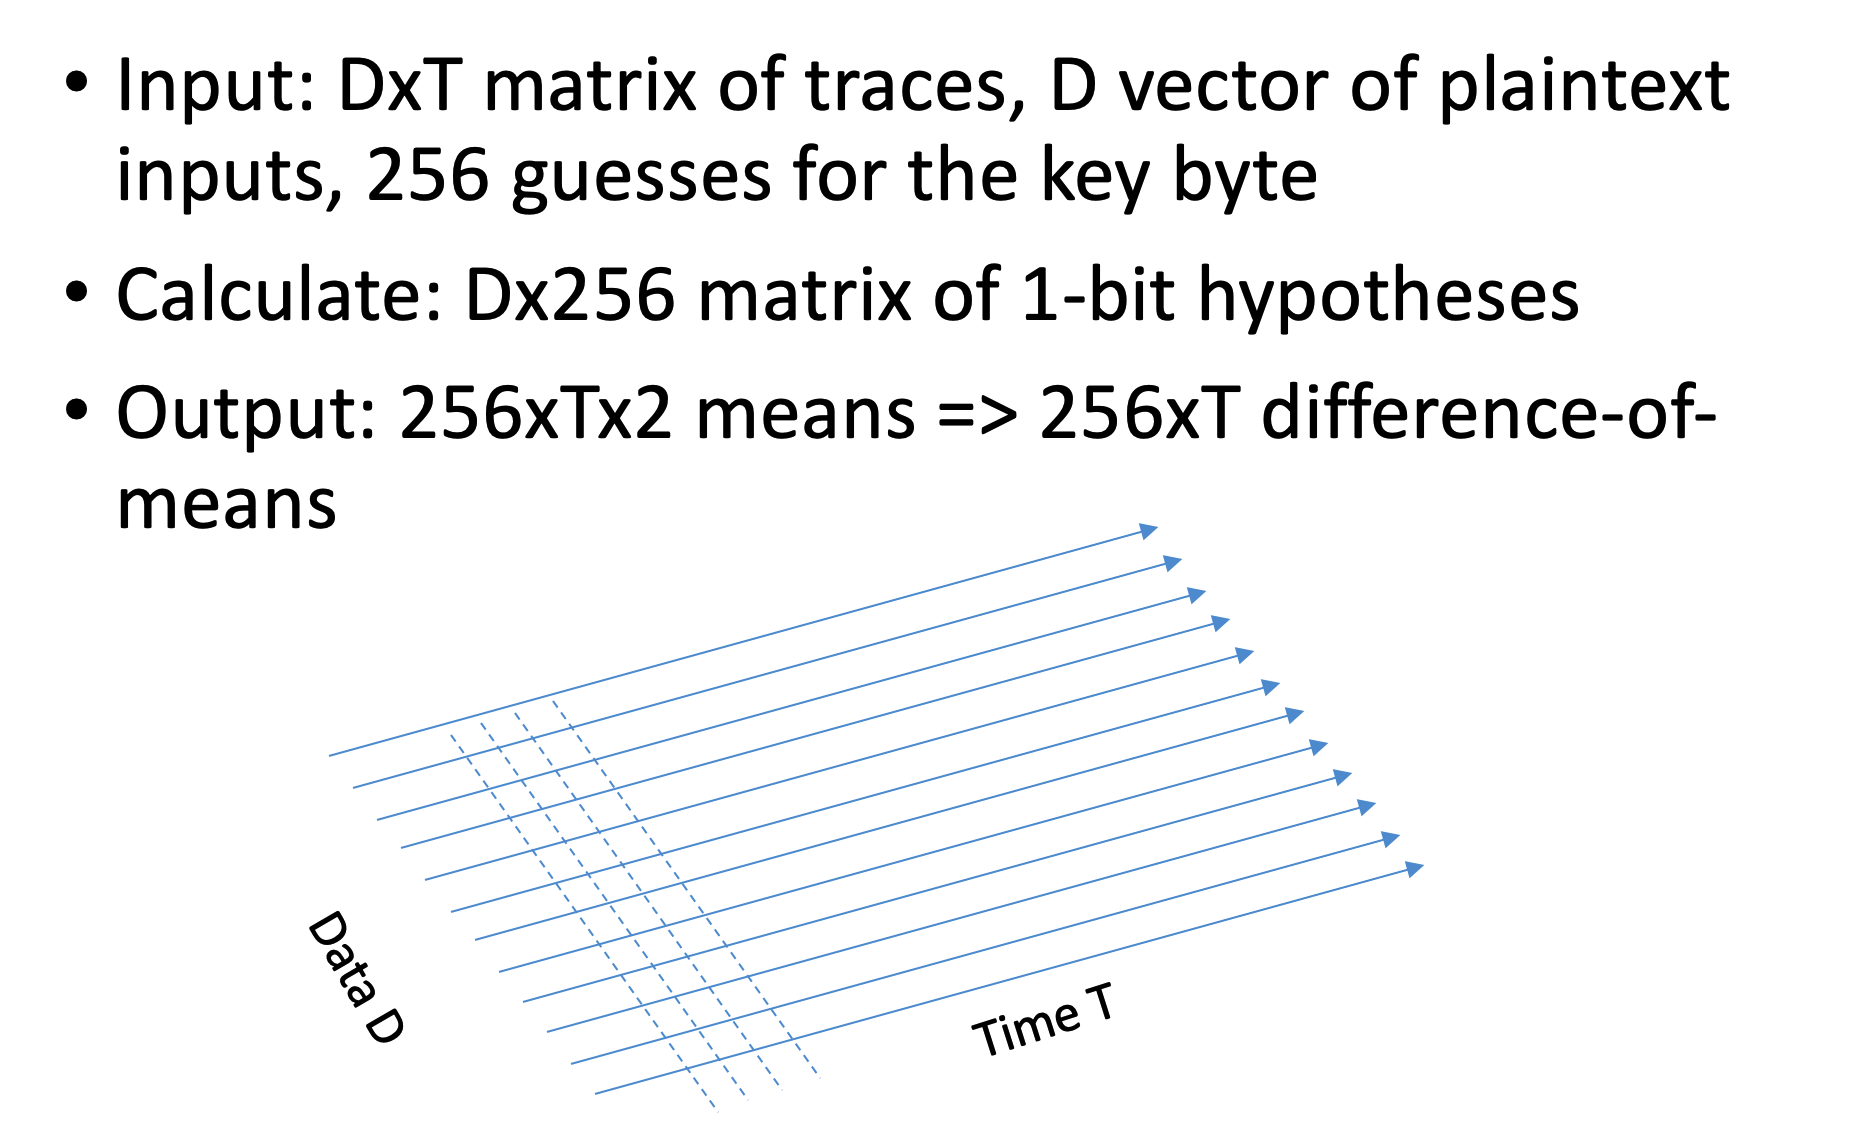
\includegraphics[width=0.8\textwidth]{images/Lecture6/dpa-separation-figure.png}
    \caption{The way we separate the data to groups based on the guess} \label{fig:dpa-separation-figure}
\end{figure}

The problem is that we have many different points on time, and we shall see a
difference only at a certain point. Therefore what we do is as follows: for each
guess, we split the measurements to 2 sets and we measure the difference between
the means of their power traces on every point of time. At most of the points,
the difference won't be significant, except to the point where the guess was
done correctly. We illustrate it at \Cref{fig:meansDiffFigure}.

\begin{figure}[!ht]
    \centering
    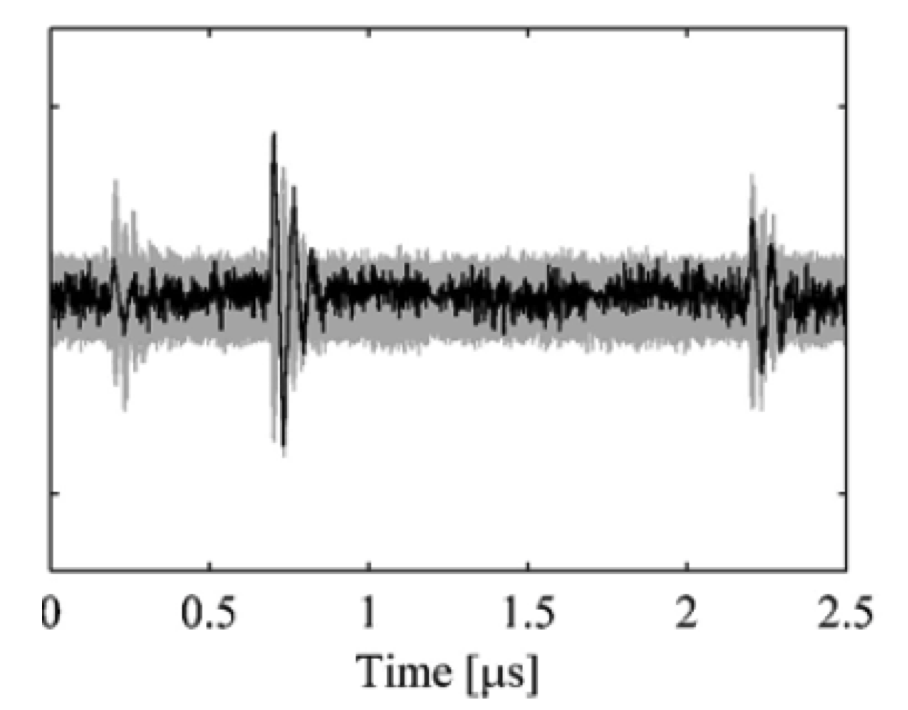
\includegraphics[width=0.8\textwidth]{images/Lecture6/meansDiffFigure.png}
    \caption{the difference of means as a function of time}
    \label{fig:meansDiffFigure}
\end{figure}

On the $X-axis$ we have the time and on the $Y-axis$ there's the difference of
means. In Gray we can see the noise and even if we guessed the correct key we
have a lot of similar points and that is because not all the times depends on
the key. But we can see in the figure the moments of peak in the means
difference, these moments are also called ``the right times". These essentially
should be the moments of the sub-bytes. If we incorrectly picked a peak which is
a ghost noise, like in a point when we xor the plain the with the key, then we
won't be able to find meaningful separation later on.

\section{DPA Lab}
In the class examp le, we attacked AES algorithm with 200 trace with size
$30,000$ using an example data from the \textit{Power Analysis Attacks} book and
we visualized the process. First, we load the data and plot it in
\Cref{fig:traceByTime} with the following axes: $X-Axis$ will be the time and
$Y-Axis$ will be the trace number. In addition, we had a dimension of color
intensity which will be depend on the power consumption.

\begin{figure}[!ht]
    \centering
    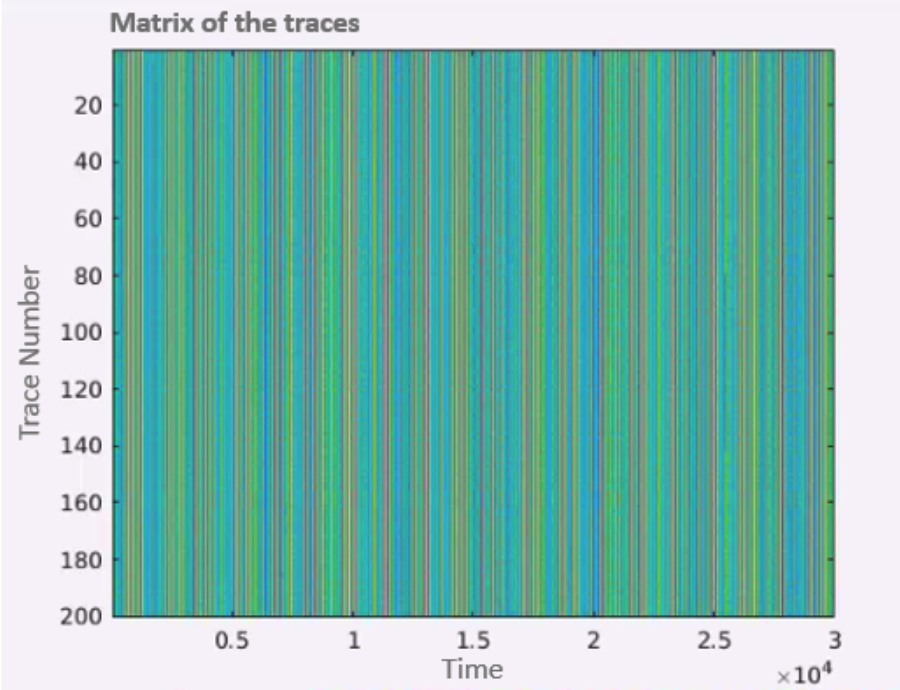
\includegraphics[width=0.8\textwidth]{images/Lecture6/traceByTime.png}
    \caption{the traces' power consumption by time} \label{fig:traceByTime}
\end{figure}

What we can see in plot \ref{fig:traceByTime} is that there are very aligned
columns which indicate that the traces are aligned properly. Our goal is to
separate the power traces of the correct key from all the other traces. To do
that, we start by showing in \Cref{fig:2traces-by-time} by comparing the power
consumption of 2 traces based on time.

\begin{figure}[!ht]
    \centering
    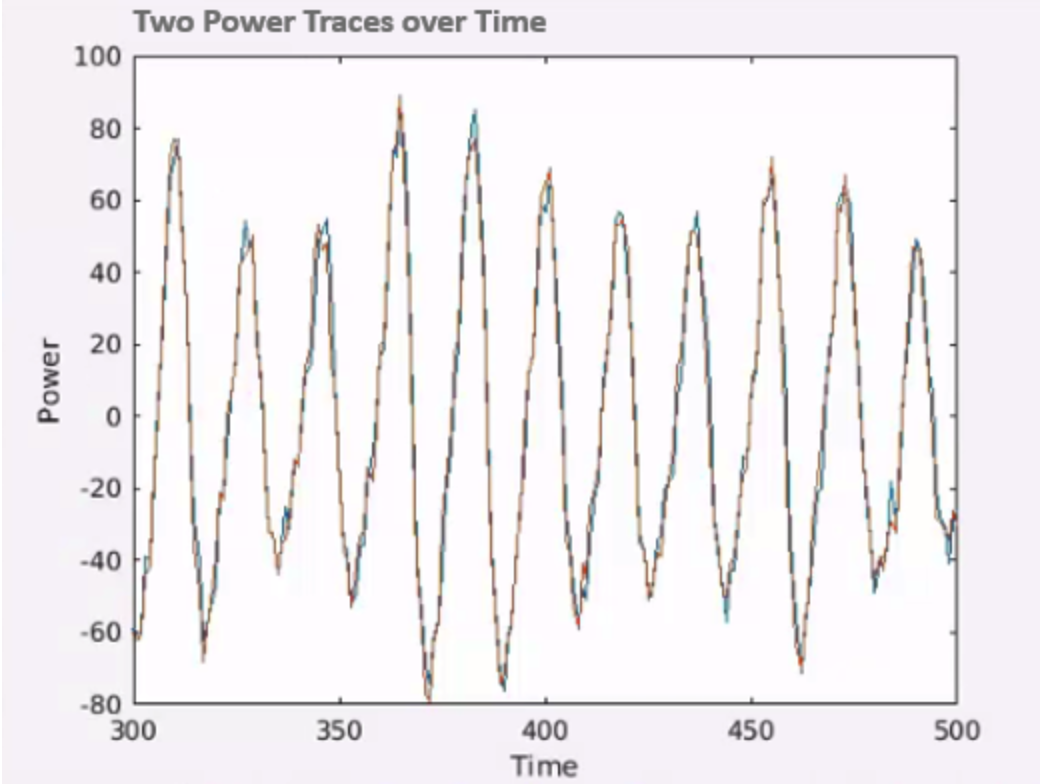
\includegraphics[width=0.8\textwidth]{images/Lecture6/2traces-by-time.png}
    \caption{2 groups of traces by times} \label{fig:2traces-by-time}
\end{figure}

We can see that both of them are overlapping, but if we had a difference between
them we would be able to find a separations on this graph.

Therefore, in \Cref{fig:intensity_by_guess} we test for each key guess and
input, what was the power consumption, whereas yellow represent less power and
blue more power.

\begin{figure}[!ht]
    \centering
    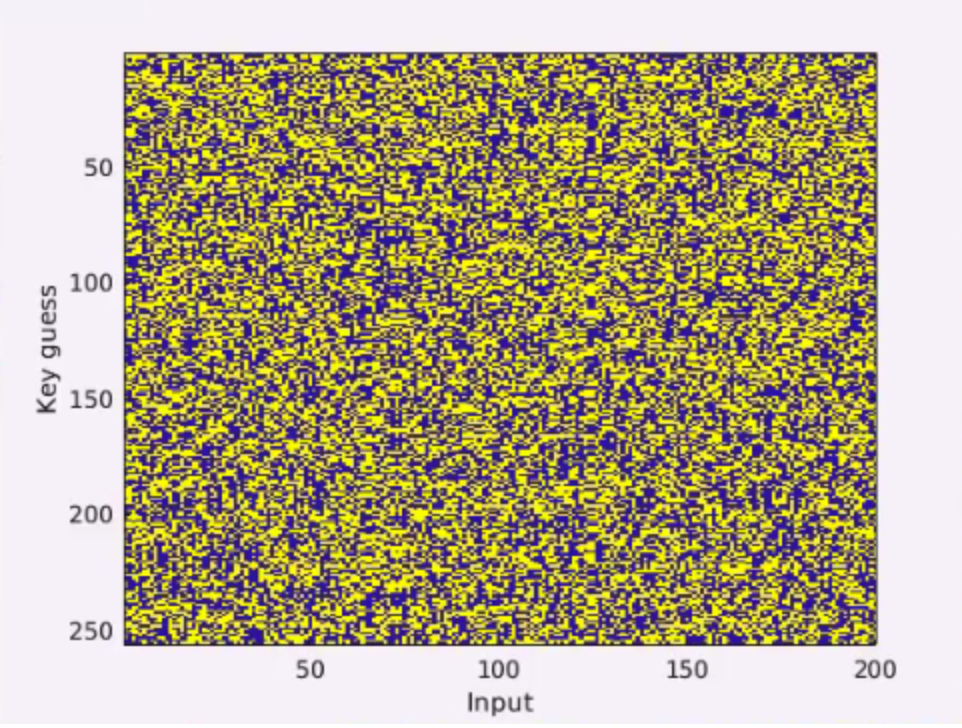
\includegraphics[width=0.8\textwidth]{images/Lecture6/intensity_by_guess.png}
    \caption{power consumption by guess and input} \label{fig:intensity_by_guess}
\end{figure}

Now we calculate the mean of power consumption for each guess and we plot if
over time

\begin{figure}[!ht]
    \centering
    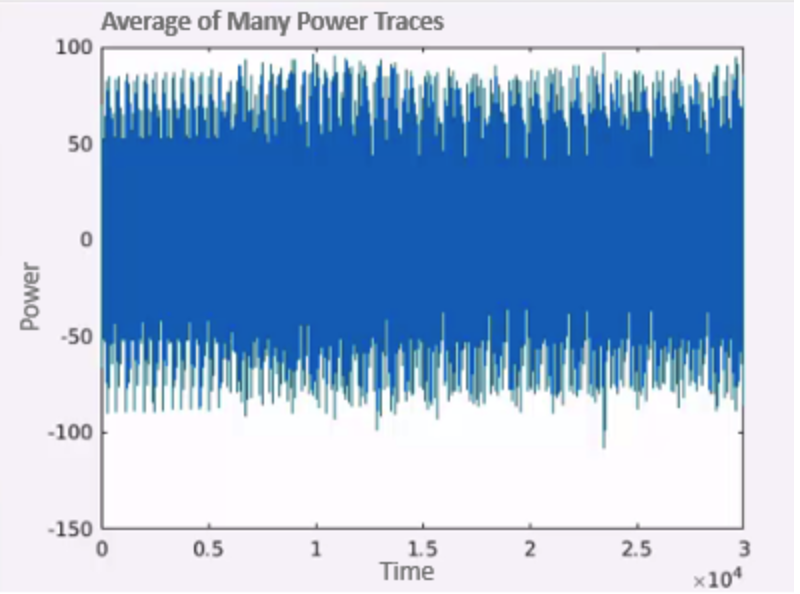
\includegraphics[width=0.8\textwidth]{images/Lecture6/avg_of_many_traces.png}
    \caption{mean of each guess across the different inputs by time} \label{fig:avg_of_many_traces}
\end{figure}

If we made the split correctly, this power trace average will be different from
all the other 255 graphs. The problem with this chart is that we need to check
many graphs, so we need something that shows the distance of means for all the
guesses. A better graph will be to plot the distance of means of each key guess
by time and then to search for the moment with the maximum difference (``the
right time") like in \Cref{fig:intensity_represents_means_diff}.

\begin{figure}[!ht]
    \centering
    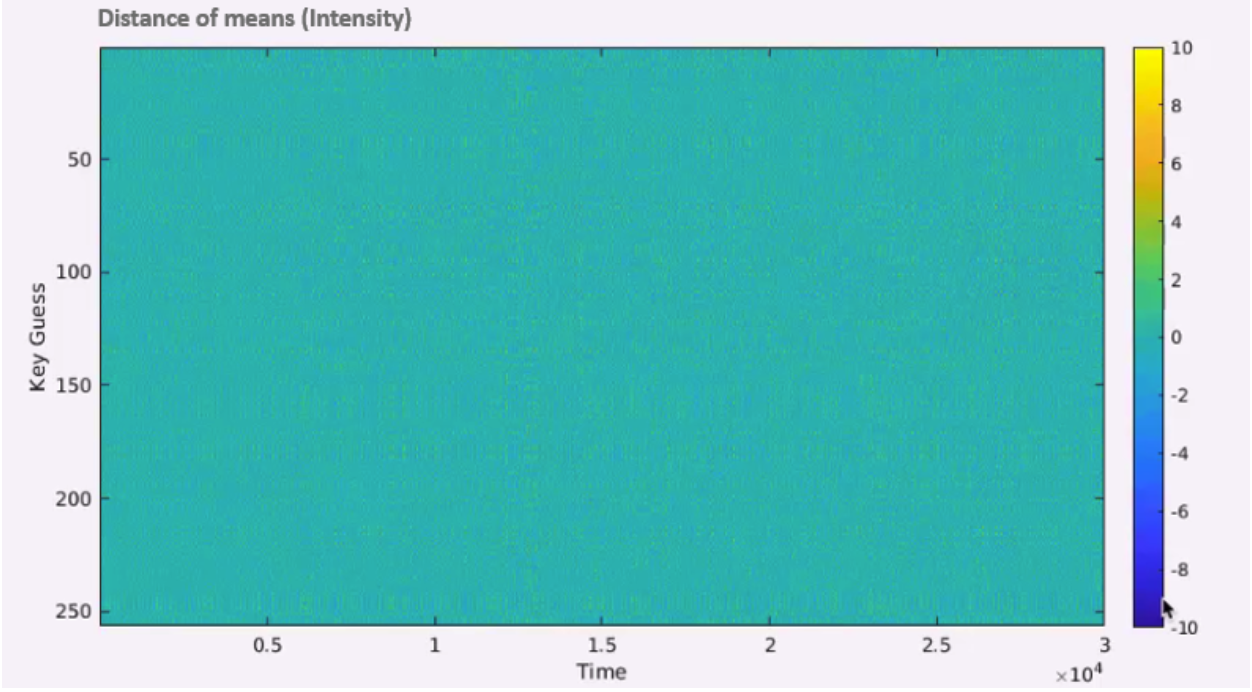
\includegraphics[width=0.8\textwidth]{images/Lecture6/intensity_represents_means_diff.png}
    \caption{distance of means by time and key guess, color intensity represents the distance} \label{fig:intensity_represents_means_diff}
\end{figure}

While it might be hard to spot it on this chart, there's a certain point of time
where the difference is $8.91$, and at all the other points it's somewhere near
0 as we can see on the charts.

What if we focus on the correct time across the different key guesses? we should
be able to spot the correct guess as shown in \Cref{fig:the-correct-time}.

\begin{figure}[!ht]
    \centering
    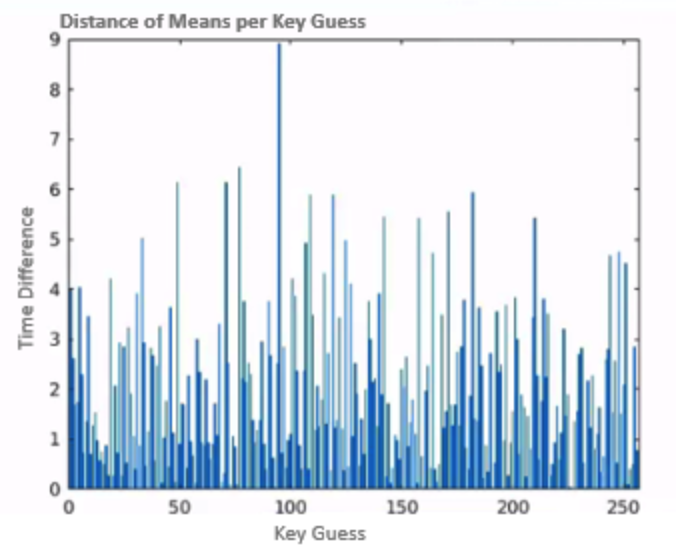
\includegraphics[width=0.8\textwidth]{images/Lecture6/the-correct-time.png}
    \caption{means distance at the correct time} \label{fig:the-correct-time}
\end{figure}

We finish by plotting the distance of means across time for all the keys, we can
see in green the distance of means for the correct key and we can see that in
the right time it's separated from the other keys as shown in \Cref{fig:all}.

\begin{figure}[!ht]
    \centering
    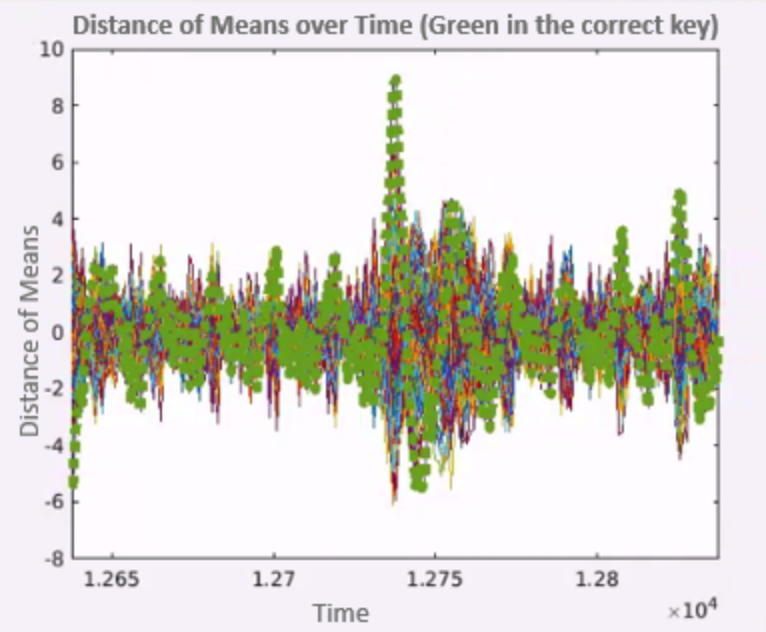
\includegraphics[width=0.8\textwidth]{images/Lecture6/all.png}
    \caption{distance of means for all key guesses across time \linebreak[4]} \label{fig:all}
\end{figure}






\subsubsection{Research Highlights}

    \begin{itemize}
        \item   This paper \cite{kocher1999differential} by Paul Kocher examines specific methods for analyzing power consumption measurements to find secret keys from tamper resistant devices.
    
        The paper presents the Differential Power Analysis subject comprehensively, its background, Simple power analysis, demonstration of DES algorithm attack, attacks on additional encryption algorithms using DPA and counter measures for DPA.
        It’s also discussed approaches for building cryptosystems that can operate securely in existing hardware that leaks information.
        \item Another article publish on 2005 \cite{mangard2005successfully} presents an attack on masked AES Hardware implementations.
        During the last years, several masking schemes for AES have
        been proposed to secure hardware implementations against DPA attacks.
        In order to investigate the effectiveness of these countermeasures in practice,
        the researchers responsible for the article designed and manufactured an ASIC. The chip features an
        unmasked and two masked AES-128 encryption engines that can be attacked
        independently.
        In addition to conventional DPA attacks on the output of registers,
        they have also mounted attacks on the output of logic gates. Based on
        simulations and physical measurements they show that the unmasked and
        masked implementations leak side-channel information due to glitches
        at the output of logic gates. It turns out that masking the AES S-Boxes does not prevent DPA attacks, if glitches occur in the circuit. However, an attacker usually does not have easy access to the back-annotated
        netlist of a product.
        \item This Article posted by Stefan Mangard \cite{mangard2004hardware}
        maintain that  Many hardware countermeasures against differential power analysis (DPA) attacks have been developed during the last years. Designers of cryptographic devices using such countermeasures to protect their devices have the challenging task to select and implement a suitable combination of countermeasures. Every device has different requirements, and so there is no universal solution to protect devices against DPA  attacks.

        In this article, a statistical approach is pursued to determine the effect of hardware countermeasures on the number of samples needed in DPA attacks. This approach results in a calculation method that enables designers to assess the resistance of their devices against DPA attacks throughout the design process. This way, different combinations of countermeasures can be easily compared and costly design iterations can be avoided.
        \item This article \cite{herbst2006aes} presents a countermeasure to Power Analysis attack on AES.
        The article describes an efficient AES software implementation that is well suited for 8-bit smart cards and resistant against power analysis attacks. Our implementation masks the intermediate results and randomizes the sequence of operations at the beginning and the end of the AES execution. Because of the masking, it is secure against simple power analysis attacks, template attacks and first-order DPA attacks. 
        Due to the combination of masking and randomization, it is resistant against higher-order DPA attacks. Resistant means that many measurements is required for a successful attack. 
        
        The implementation shown in the article compares well with other protected and unprotected AES software implementations for smart cards. The practical attacks that we have performed support our theoretical estimates about the security of the countermeasures.
        This article also includes a practical evaluation of the countermeasures. The results prove the theoretical assessment of the countermeasures to be correct.
    \end{itemize}

  



